\section{Aplicación propuesta}

% Arquitectura General
\begin{frame}{Arquitectura General}
  Separación física y lógica entre Front-End y Back-End
  \begin{itemize}
    \item Conectados entre sí por una red interna
  \end{itemize}
  Ventajas
  \begin{itemize}
    \item Un mismo Front-End puede comunicarse con varios Back-End
    \item Back-End aislado, no accesible directamente desde el exterior
    \item Interfaz disponible aun cuando el Back-End no está operativo
  \end{itemize}
  \begin{figure}
    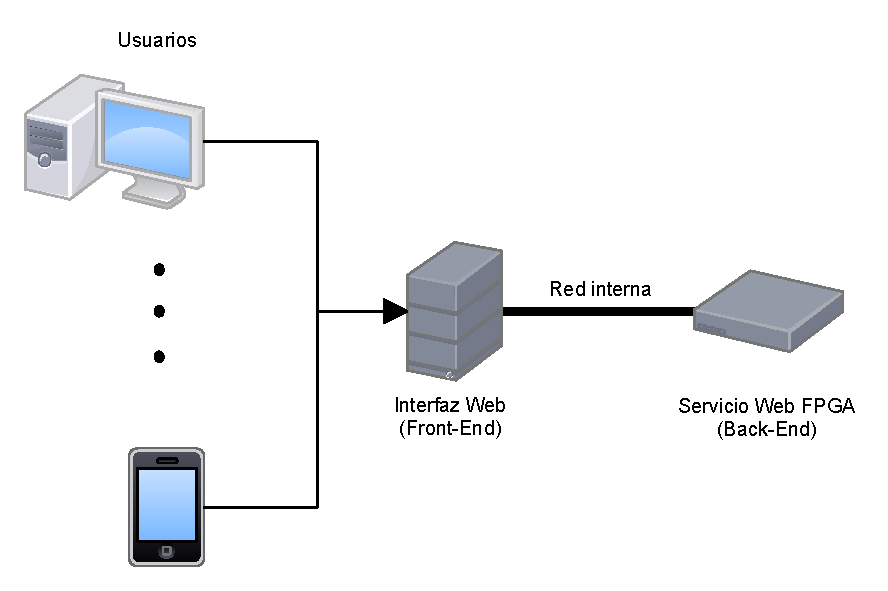
\includegraphics[width=0.5\linewidth]{arquitectura}
  \end{figure}
\end{frame}

% Stack de tecnologías
\begin{frame}{Stack tecnológico}
  \begin{itemize}
    \item Back-End
    \begin{itemize}
      \item JavaScript
      \item node.js
      \item express, async, nodemon
    \end{itemize}
    \item Front-End
    \begin{itemize}
      \item PHP (HTML, JavaScript, CSS)
      \item Framework propio
      \item Bootstrap, jQuery
    \end{itemize}
  \end{itemize}
\end{frame}

% Back-End
\begin{frame}{Back-End - Servicio Web FPGA}
  \begin{itemize}
    \item Formalizar y exponer la funcionalidad de la FPGA
    \item Permite conocer el estado de la misma y de aspectos relacionados
    \item Implementación REST-like
  \end{itemize}
  \begin{figure}
    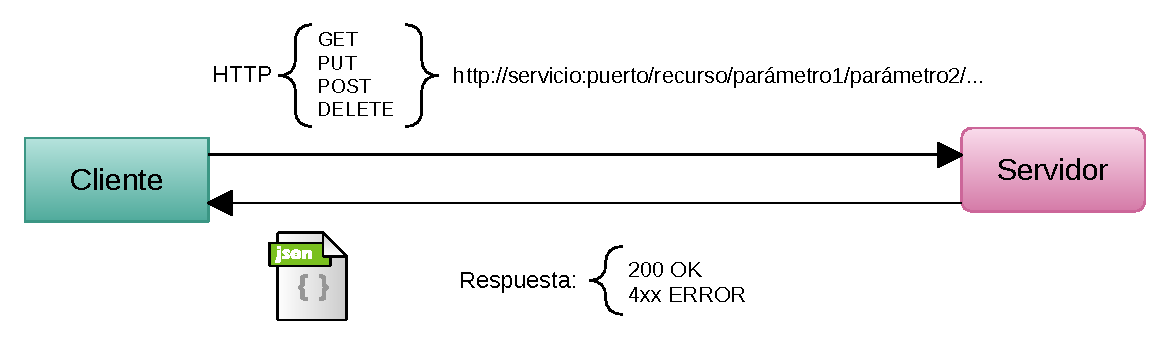
\includegraphics[width=\linewidth]{fpga_rest}
  \end{figure}
\end{frame}

\begin{frame}{Back-End - Arquitectura interna}
  \begin{figure}
    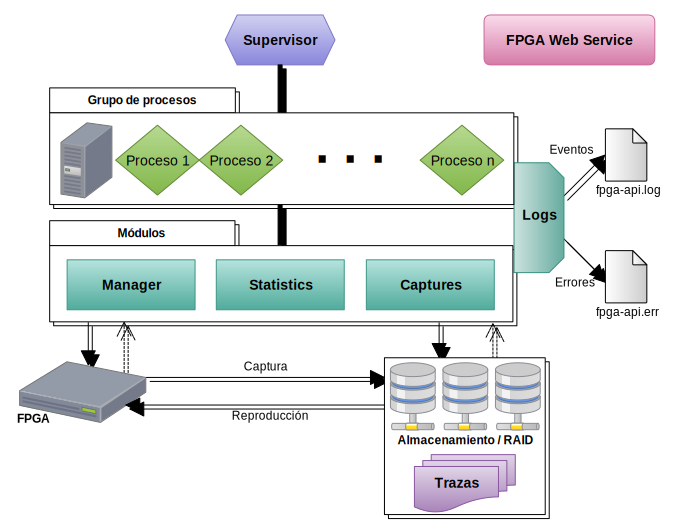
\includegraphics[width=0.85\linewidth]{fpga}
  \end{figure}
\end{frame}

\begin{frame}{Back-End - FSM Estado FPGA}
  \begin{itemize}
    \item Formaliza el estado de la FPGA de forma no persistente
  \end{itemize}
  \begin{figure}
    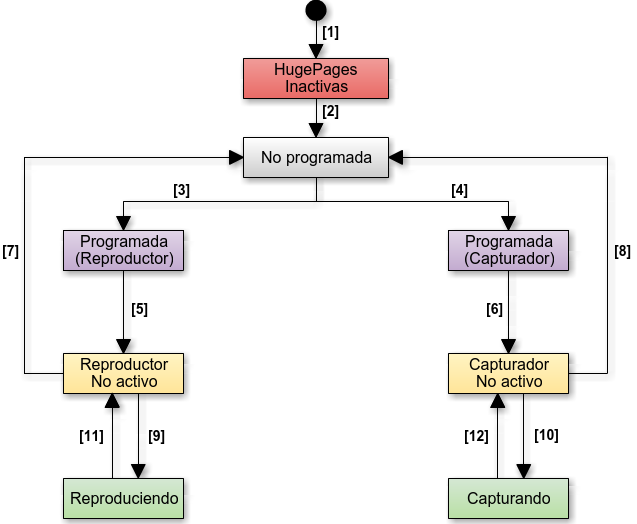
\includegraphics[width=0.65\linewidth, valign=t]{fpga_estado}
    \hfill
    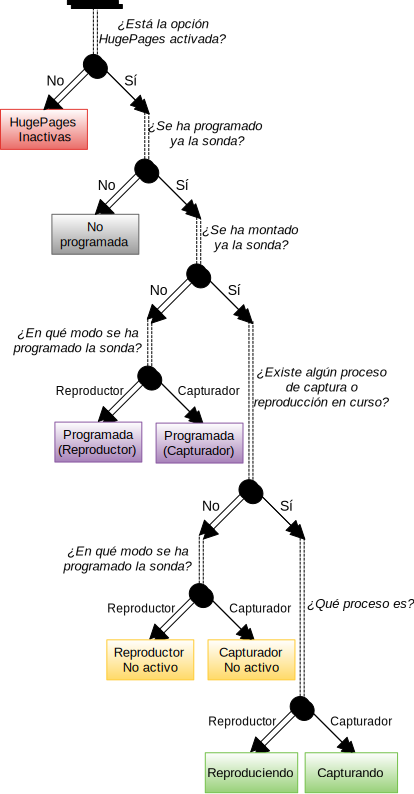
\includegraphics[height=0.7\textheight, valign=t]{arbol_decision_vertical}
  \end{figure}
\end{frame}

\begin{frame}{Back-End - API REST-like}
  \begin{itemize}
    \item API REST-like - Métodos accesibles por HTTP
  \end{itemize}
  \begin{figure}
    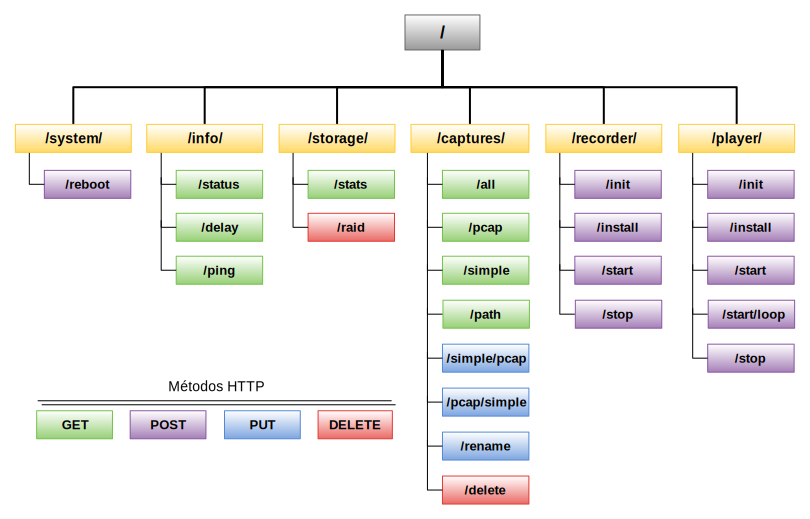
\includegraphics[width=0.9\linewidth]{arbol_metodos}
  \end{figure}
\end{frame}

% Front-End
\begin{frame}{Front-End - Framework - Arquitectura interna}
  Framework propio
  \begin{itemize}
    \item Únicamente la funcionalidad necesaria
    \item Mayor control sobre el funcionamiento interno del mismo
  \end{itemize}
  \begin{figure}
    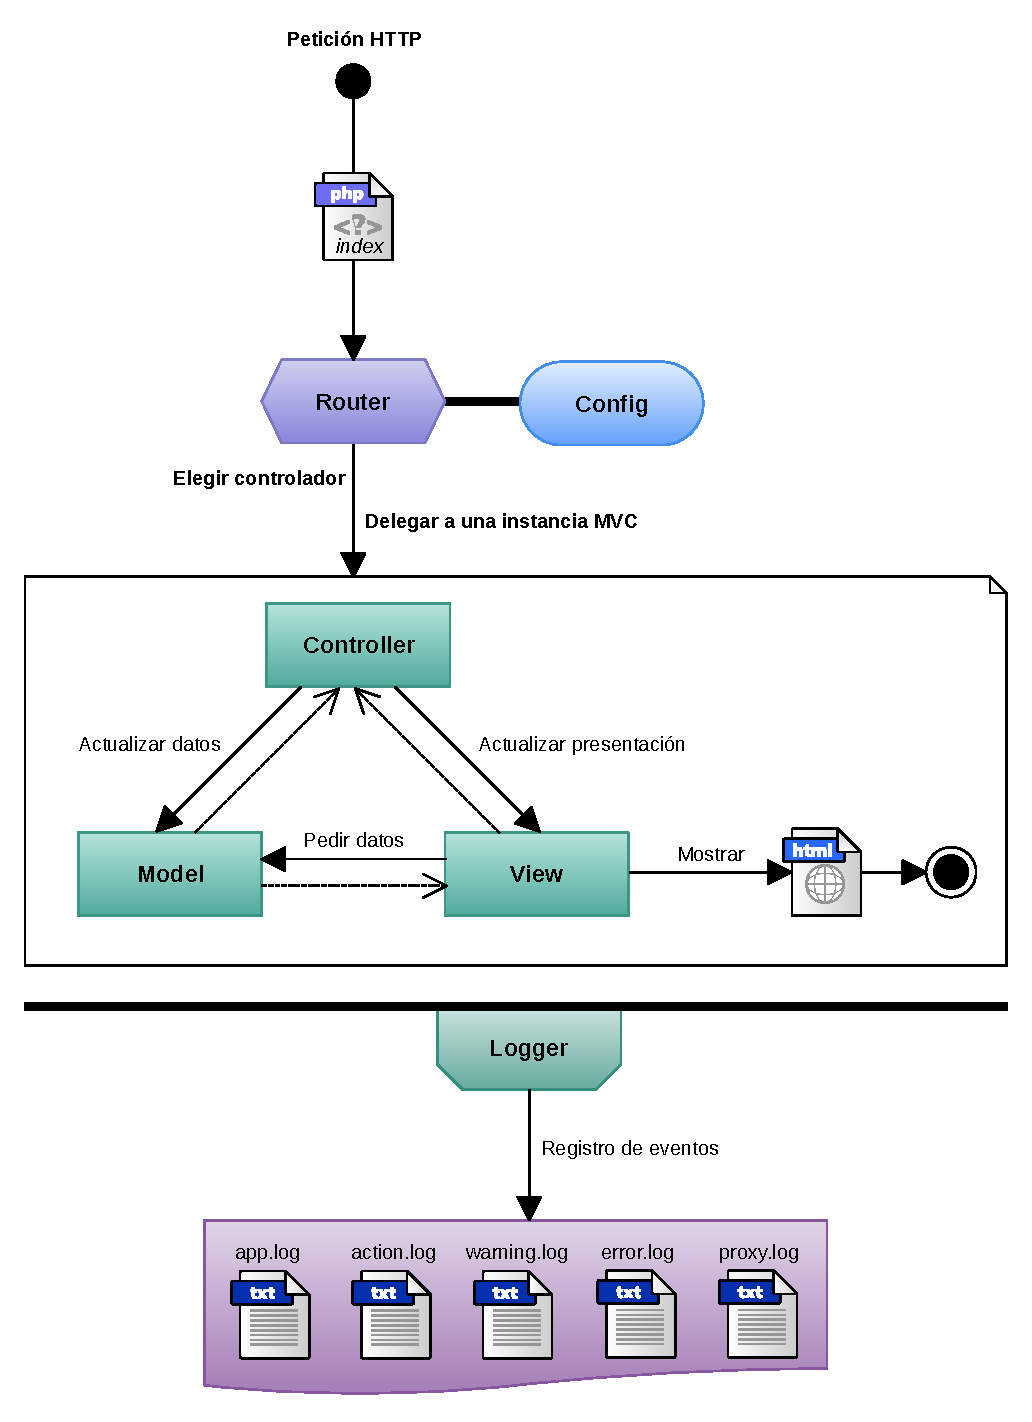
\includegraphics[width=\linewidth]{framework}
  \end{figure}
\end{frame}

\begin{frame}{Front-End - Framework - Router}
  \begin{itemize}
    \item Carga el módulo/método correspondiente para cada petición HTTP
  \end{itemize}
  \begin{figure}
    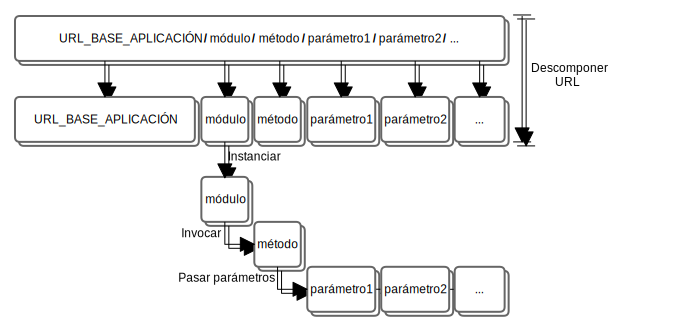
\includegraphics[width=\linewidth]{router}
  \end{figure}
\end{frame}

\begin{frame}{Front-End - Framework - Proxy}
  \begin{itemize}
    \item Comunicación con el Servicio Web FPGA
  \end{itemize}
  \begin{figure}
    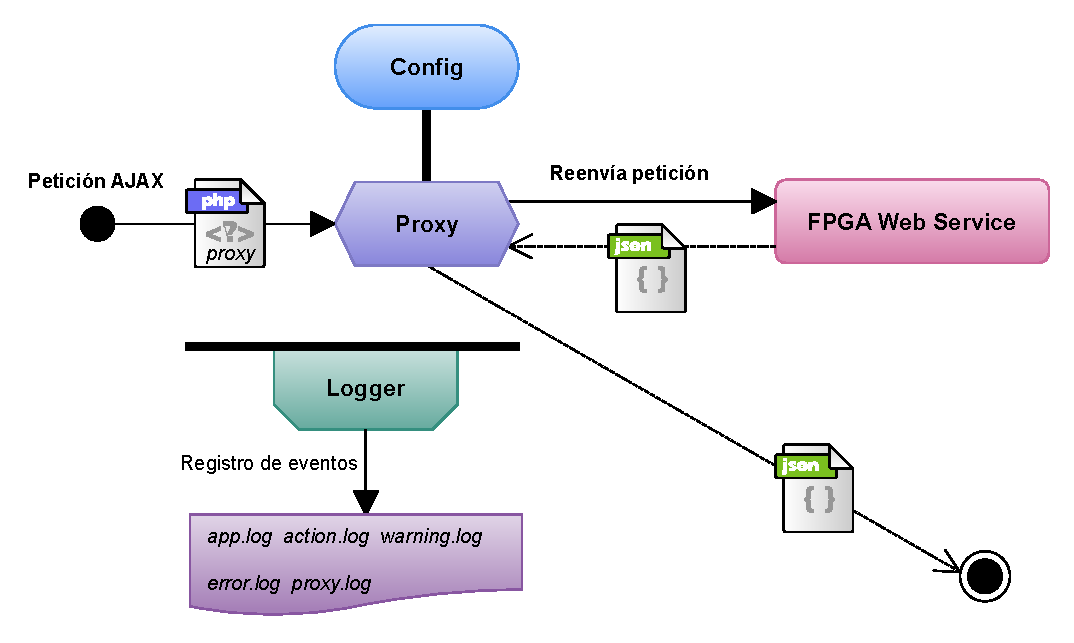
\includegraphics[width=\linewidth]{proxy}
  \end{figure}
\end{frame}

\begin{frame}{Front-End - Diseño - Capturas}
  \begin{figure}
    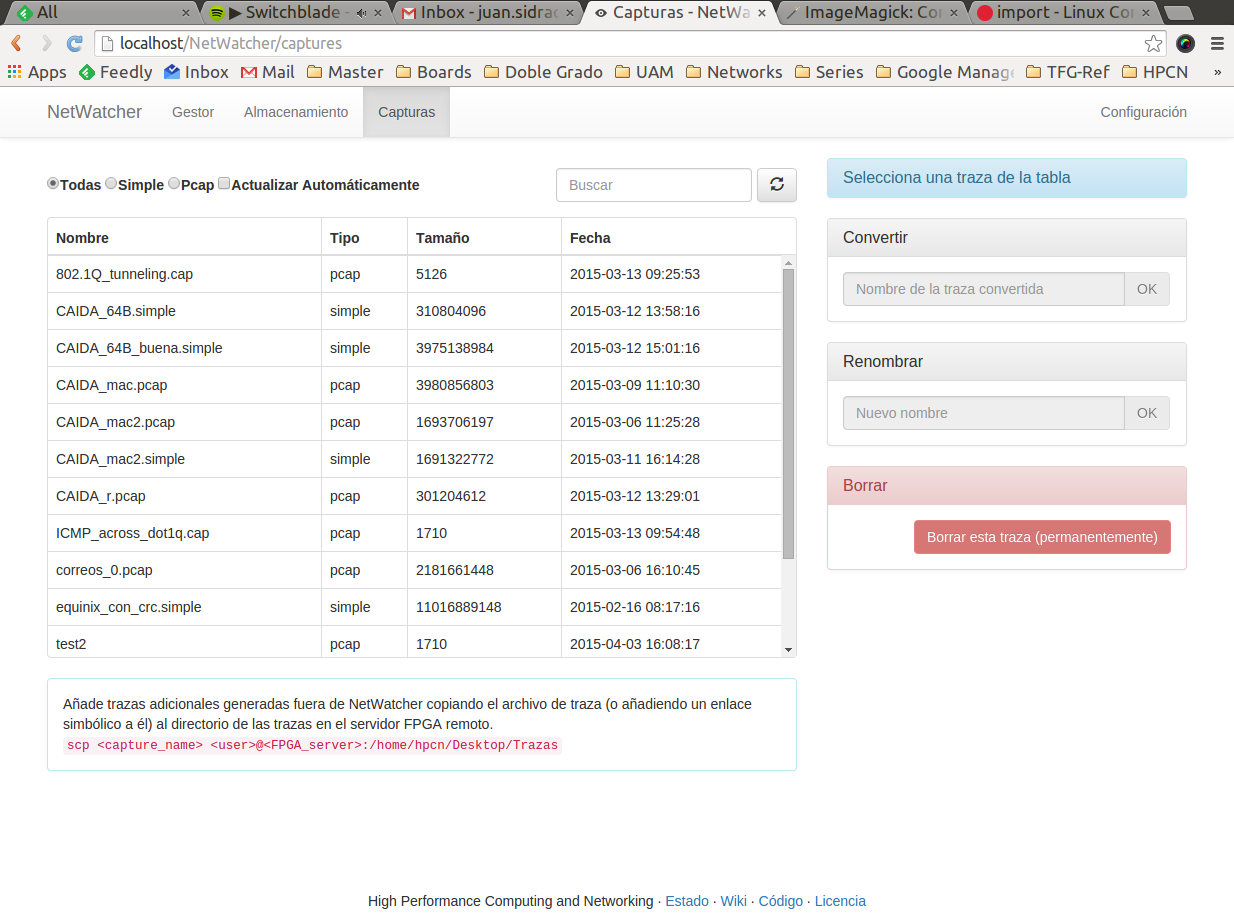
\includegraphics[width=\linewidth]{capturas}
  \end{figure}
\end{frame}

\begin{frame}{Front-End - Diseño - Gestor reproducción}
  \begin{figure}
    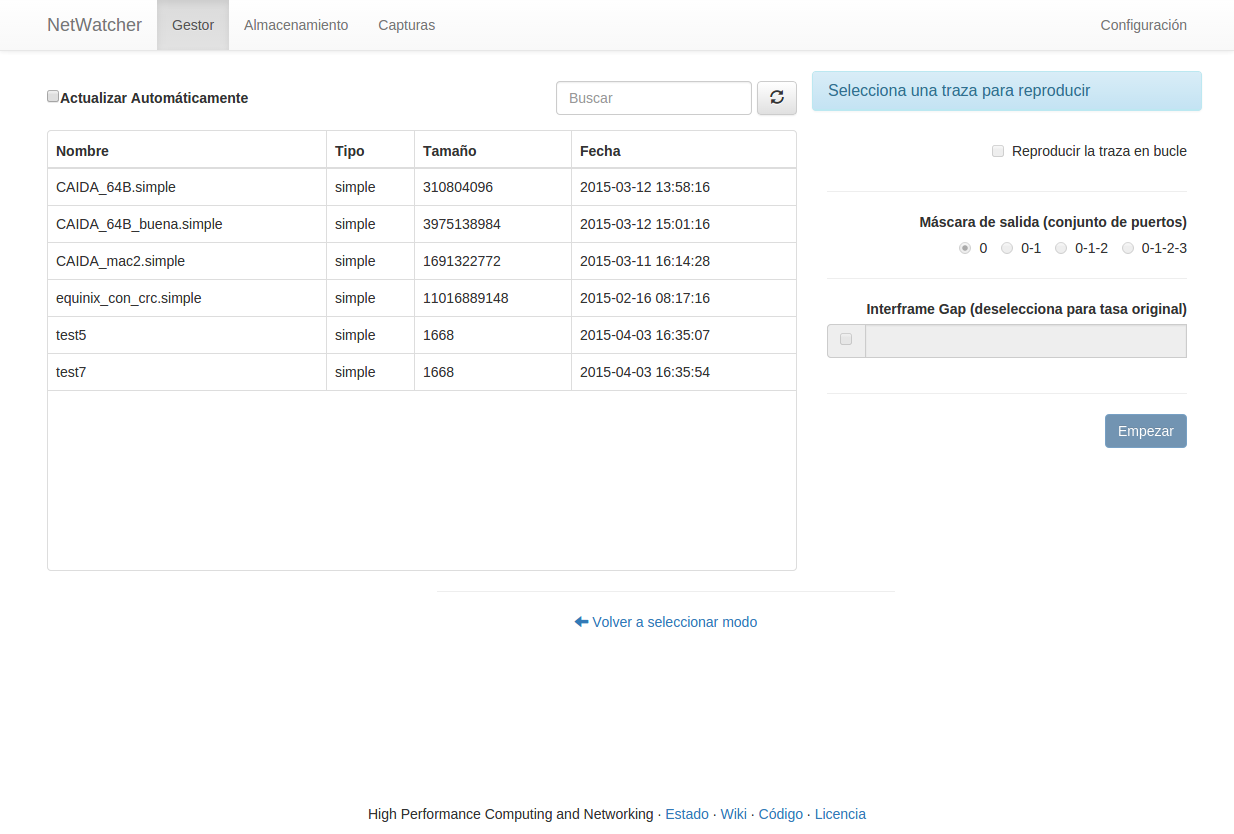
\includegraphics[width=\linewidth]{gestor_reproducir}
  \end{figure}
\end{frame}

\begin{frame}{Front-End - Diseño - Estado}
  \begin{itemize}
    \item Diseño \textit{responsive} - adaptado a cada dispositivo
  \end{itemize}
  \begin{figure}
    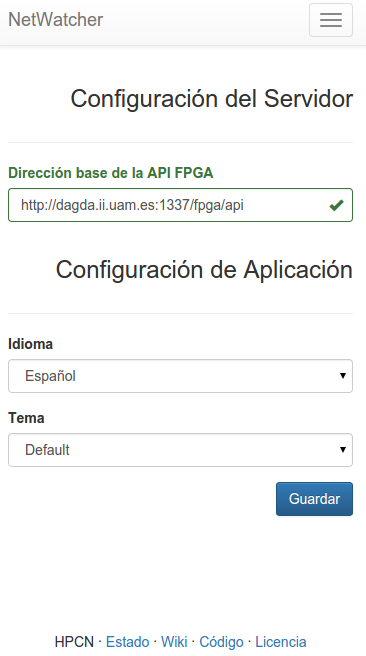
\includegraphics[width=0.3\linewidth, valign=t]{configuracion_movil}
    \hfill
    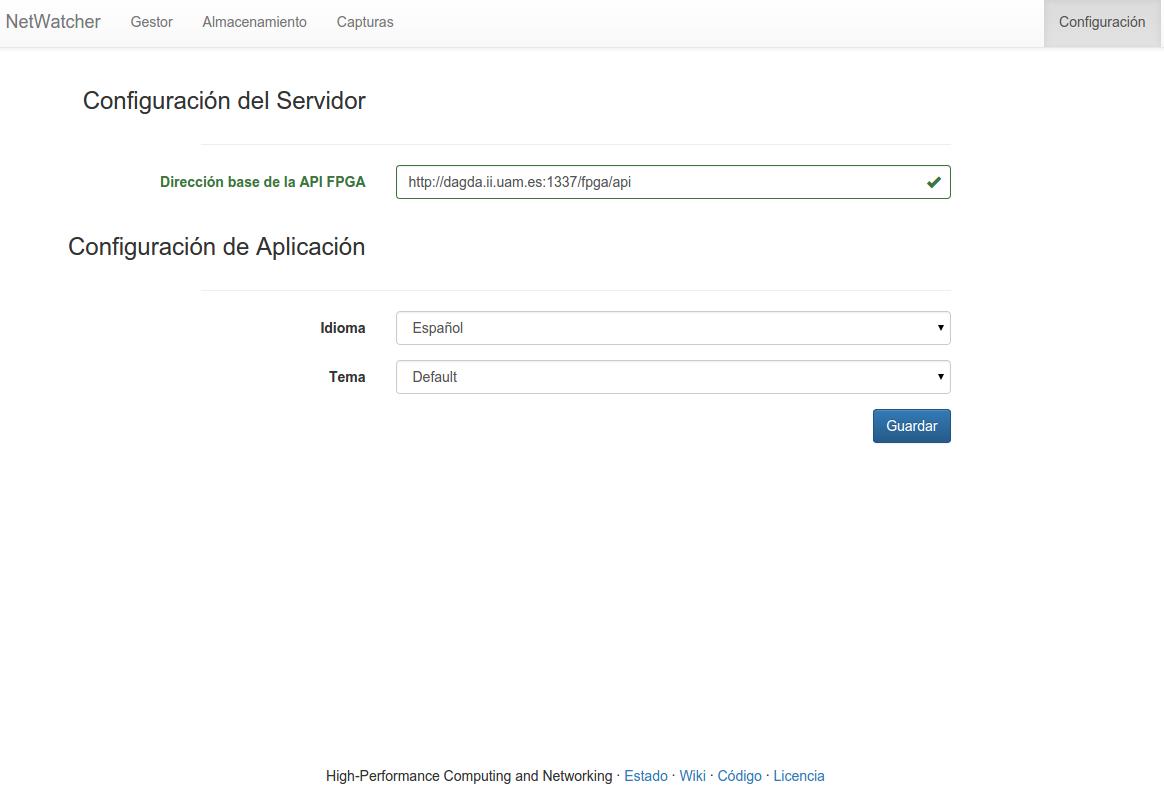
\includegraphics[width=0.65\linewidth, valign=t]{configuracion_pc}
  \end{figure}
\end{frame}
